\documentclass{standalone}
\usepackage{tikz}
\usetikzlibrary{positioning,automata}
\begin{document}
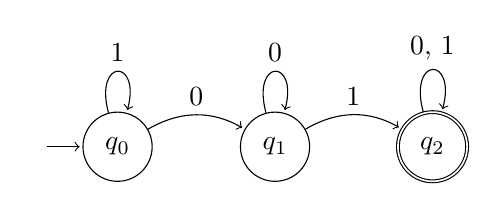
\begin{tikzpicture}[shorten >=1pt, node distance=2cm, on grid]
  \node[state, initial, initial text=] (q0) {$q_0$};
  \node[state] (q1) [right=of q0] {$q_1$};
  \node[state, accepting] (q2) [right=of q1] {$q_2$};
  \path[->] (q0) edge[loop above] node{1} (q0)
            (q1) edge[loop above] node{0} (q1)
            (q2) edge[loop above] node{0, 1} (q2)
            (q0) edge[bend left, above] node{0} (q1)
            (q1) edge[bend left, above] node{1} (q2);
\end{tikzpicture}
\end{document}